\documentclass{beamer}
\usepackage{tikz}
\usepackage[all]{xy}
\usepackage{amsmath,amssymb}
\usepackage{hyperref}
\usepackage{graphicx}
\usepackage{algorithmic}
\usepackage{multirow}

\DeclareMathOperator*{\argmin}{arg\,min}
\DeclareMathOperator*{\Lik}{Lik}
\DeclareMathOperator*{\PoissonLoss}{PoissonLoss}
\DeclareMathOperator*{\Peaks}{Peaks}
\DeclareMathOperator*{\Segments}{Segments}
\DeclareMathOperator*{\argmax}{arg\,max}
\DeclareMathOperator*{\maximize}{maximize}
\DeclareMathOperator*{\minimize}{minimize}
\newcommand{\sign}{\operatorname{sign}}
\newcommand{\RR}{\mathbb R}
\newcommand{\ZZ}{\mathbb Z}
\newcommand{\NN}{\mathbb N}
\newcommand{\z}{$z = 2, 4, 3, 5, 1$} 

\newcommand{\algo}[1]{\textcolor{#1}{#1}}
\definecolor{PDPA}{HTML}{66C2A5}
\definecolor{CDPA}{HTML}{FC8D62}
\definecolor{GPDPA}{HTML}{4D4D4D}

% Set transparency of non-highlighted sections in the table of
% contents slide.
\setbeamertemplate{section in toc shaded}[default][100]
\AtBeginSection[]
{
  \setbeamercolor{section in toc}{fg=red} 
  \setbeamercolor{section in toc shaded}{fg=black} 
  \begin{frame}
    \tableofcontents[currentsection]
  \end{frame}
}

\begin{document}

\title{Introduction to machine learning and neural networks, with an application to earth system modeling}

\author{
  Toby Dylan Hocking\\
  toby.hocking@nau.edu\\
  toby.hocking@r-project.org\\
}

\maketitle

\section{Introduction and overview}

\begin{frame}
  \frametitle{Machine learning intro: image classification example}
  ML is all about learning predictive functions $f(x)\approx y$, where 
  \begin{itemize}
  \item Inputs/features $x$ can be easily computed using traditional
    algorithms. For example, matrix of pixel intensities in an image.
  \item Outputs/labels $y$ are what we want to predict, typically more
    difficult/costly to measure than inputs. For example, to get an
    image class label, you may have to ask a human. 
  \item Input $x$ = image of digit, output $y\in\{0,1,\dots,9\}$, \\--
    this is a classification problem with 10 classes.\\
  $f(
\includegraphics[height=1cm]{mnist-0})=0$,
  $f(
\includegraphics[height=1cm]{mnist-1})=1$
\item Traditional/unsupervised algorithm: I give you a pixel intensity matrix
  $x\in\RR^{28\times 28}$, you code a function $f$ that returns one of
  the 10 possible digits. Q: how to do that?
  \end{itemize}
\end{frame}

\begin{frame}
  \frametitle{Supervised machine learning algorithms}

  I give you a training data set with paired inputs/outputs, e.g.

  \begin{center}
    \Huge 0 1 2 3 4 5 6 7 8 9

  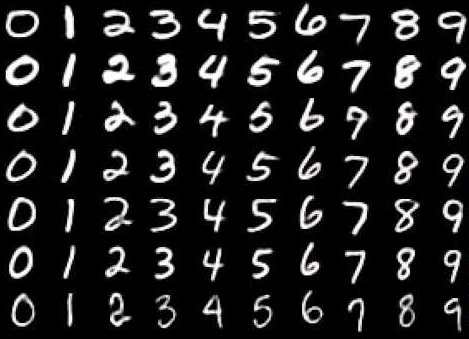
\includegraphics[height=1.9in]{mnist-digits}
  \end{center}

  Your job is to code an algorithm, \textsc{Learn}, that infers a
  function $f$ from the training data. (you don't code $f$)
  
  \scriptsize Source: github.com/cazala/mnist
\end{frame}


\begin{frame}
  \frametitle{Advantages of supervised machine learning}

  \begin{center}
    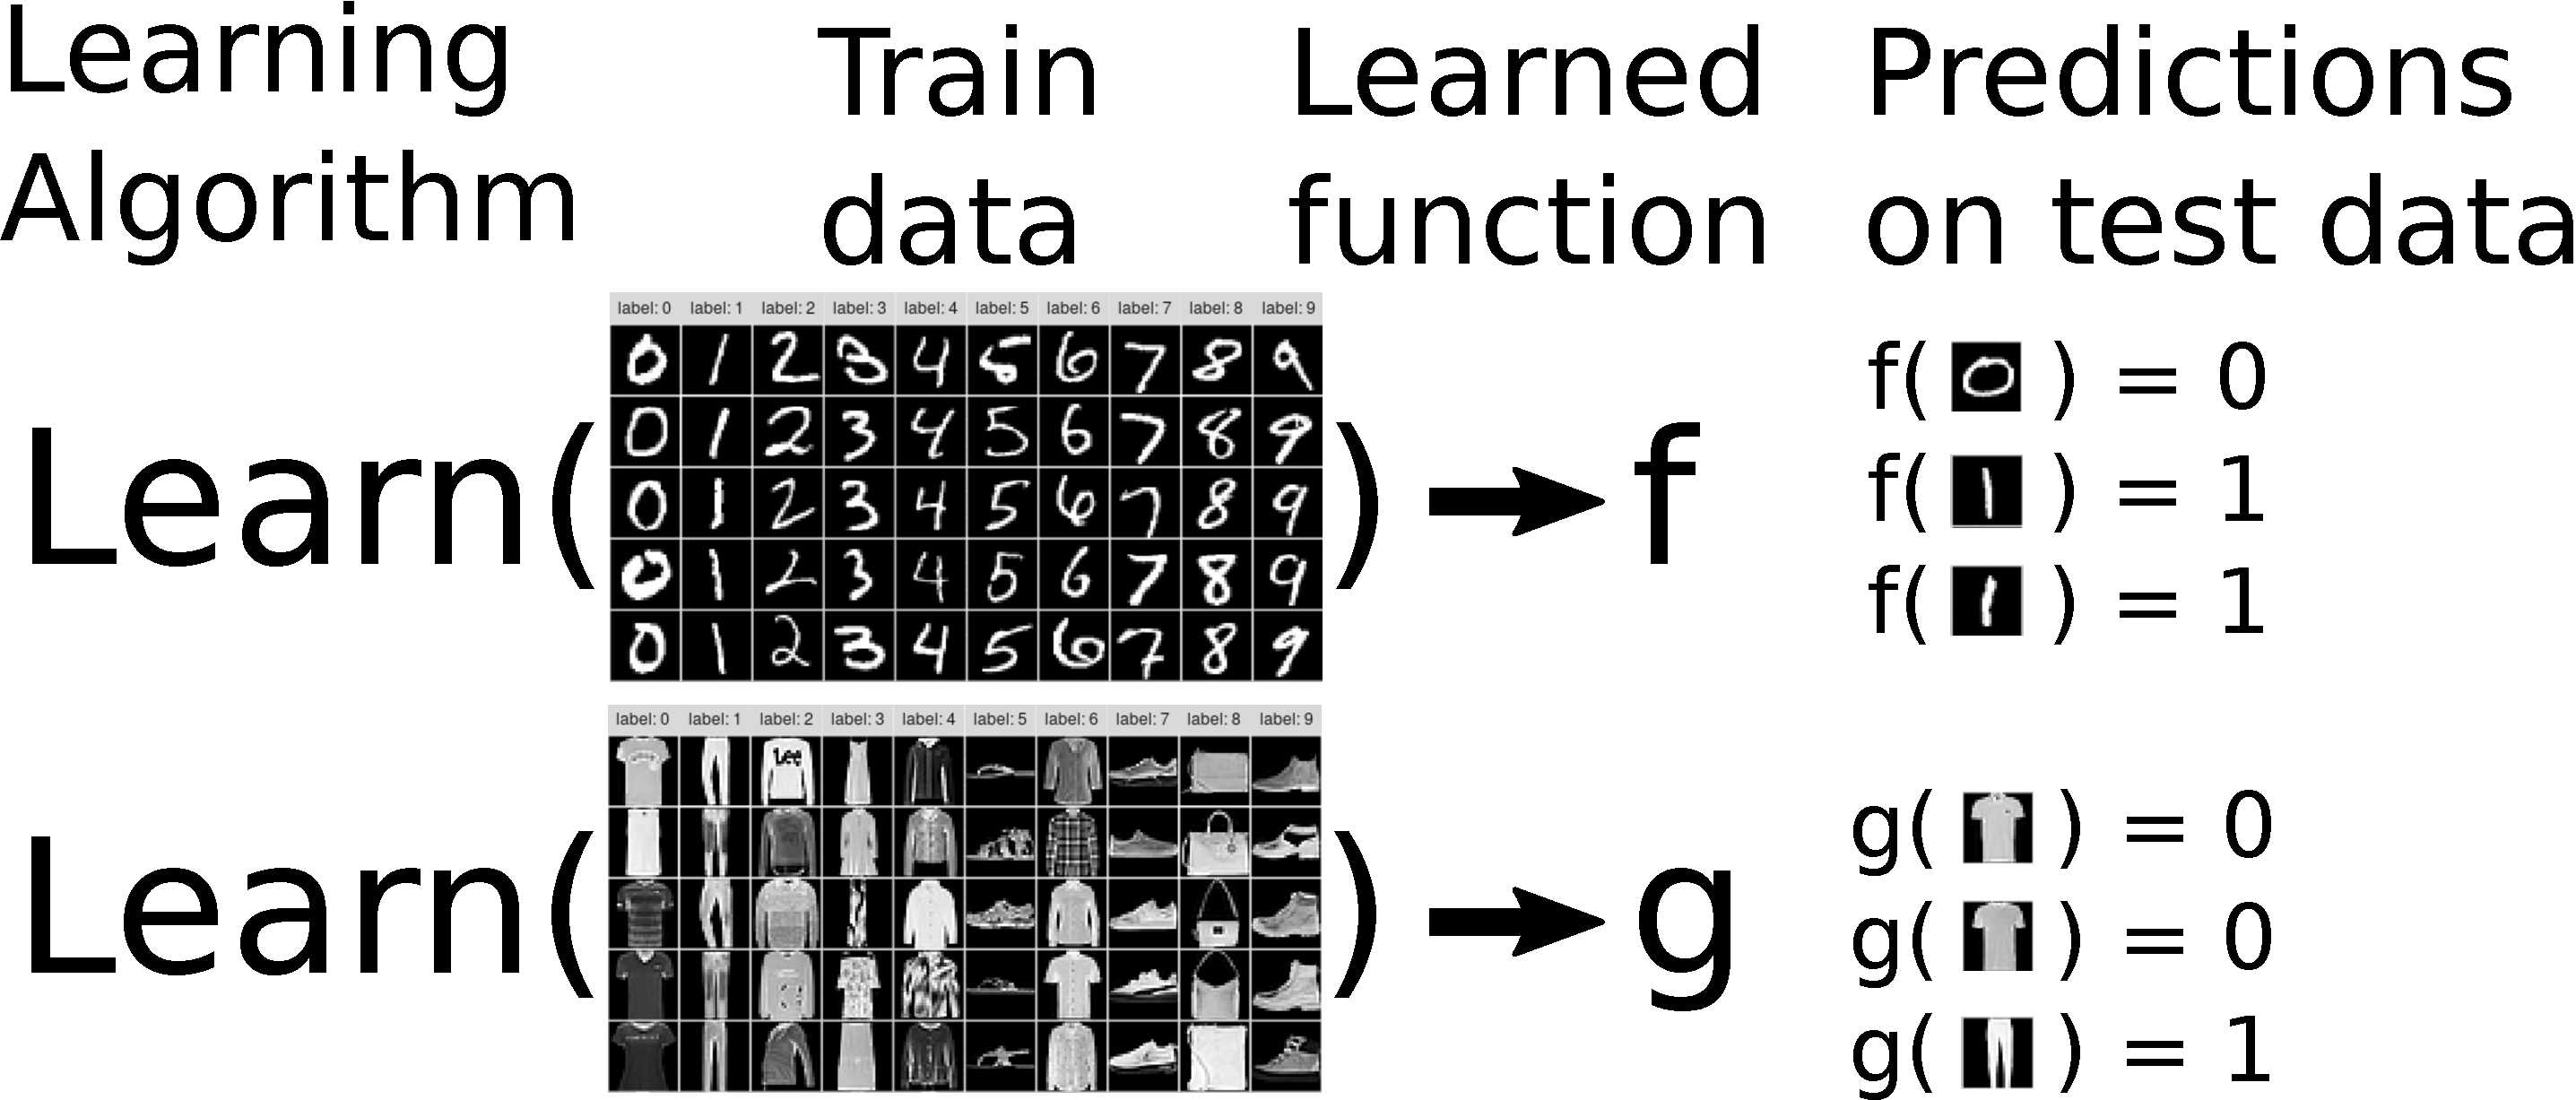
\includegraphics[width=0.8\textwidth]{drawing-mnist-train-test.pdf}
  \end{center}
  \vskip -0.2cm
  
  \begin{itemize}
  \item Input $x\in\RR^{28\times 28}$, output $y\in\{0,1,\dots,9\}$
    types the same!
  \item Can use same learning algorithm regardless of pattern.
  \item Pattern encoded in the labels (not the algorithm).
  \item Useful if there are many un-labeled data, but few labeled data
    (or getting labels is long/costly).
  \item State-of-the-art accuracy (if there is enough training data).
  \end{itemize}

  \scriptsize Sources: github.com/cazala/mnist, github.com/zalandoresearch/fashion-mnist

\end{frame}

\begin{frame}
  \frametitle{Overview of tutorial}
  In this tutorial we will discuss two kinds of problems, which
  differ by the type of the output/label/y variable we want to predict.
  \begin{itemize}
  \item Regression, y is a real number.
  \item Classification, y is an integer representing a category.
  \end{itemize}

  The rest of the tutorial will focus on three examples:
  \begin{enumerate}
  \item Regression with a single input, to demonstrate how to avoid
    overfitting.
  \item Classification of digit images, to demonstrate how to compare
    machine learning algorithms in terms of test/prediction accuracy.
  \item Regression for predicting earth system model parameters, as a
    relevant application.
  \end{enumerate}
\end{frame}

\section{Example 1: avoiding overfitting in regression
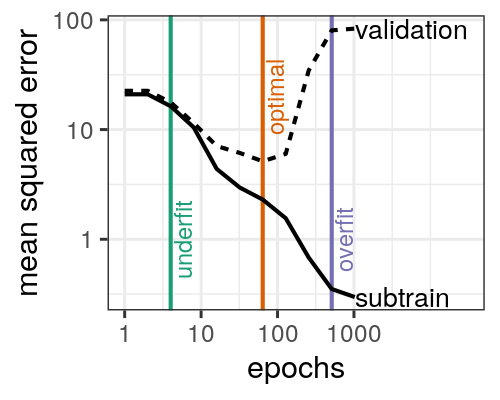
\includegraphics[height=2cm]{figure-overfitting-paper-loss}}  
 
\begin{frame}
  \frametitle{Goal of this section: demonstrate how to avoid
    overfitting}
  \begin{itemize}
  \item The goal of supervised machine learning is to get accurate
    predictions on new/unseen/held-out test data.
  \item Any machine learning algorithm is prone to overfit, which
    means providing better predictions on the train/subtrain set than
    on a held-out validation/test set. (BAD)
  \item To learn a model which does NOT overfit (GOOD), you need to
    first divide your train set into subtrain/validation sets.
  \item Code for figures in this section:
    \url{https://github.com/tdhock/2020-yiqi-summer-school/blob/master/figure-overfitting.R}
  \end{itemize}
\end{frame}

\begin{frame}
  \frametitle{Three different data sets/patterns}
  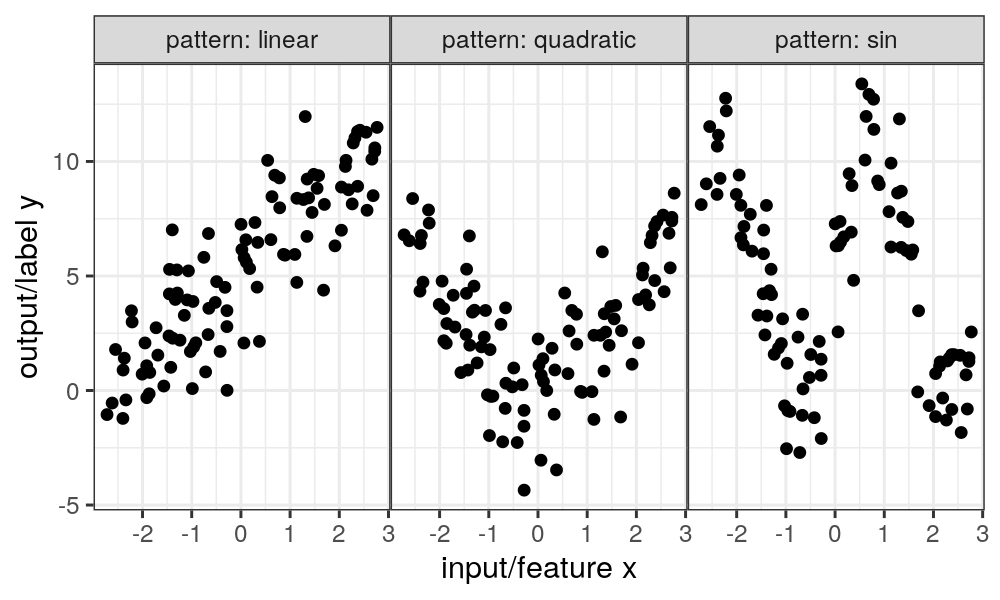
\includegraphics[width=\textwidth]{figure-overfitting-data}

  \begin{itemize}
   \item We illustrate this using a single input/feature
    $x\in\mathbb R$.
  \item We use a regression problem with outputs $y\in\mathbb R$.
  \item Goal is to learn a function $f(x)\in\mathbb R$.
  \end{itemize}
\end{frame}

\begin{frame}
  \frametitle{Neural network prediction function}
\begin{equation}
  f(\mathbf x) = f_L[\cdots f_1[\mathbf x] ].
\end{equation}
  With $L-1$ hidden layers, we have for all $l\in\{1,\dots,L\}$:
\begin{equation}
  f_l(t) = A_l( \mathbf W_l^\intercal t ),
\end{equation}
The hyper-parameters which must be fixed prior to learning:
\begin{itemize}
\item Number of layers $L$.
\item Activation functions $A_l$ (classically sigmoid, typically ReLU).
\item Number of hidden units per layer ($u_1,\dots,u_{L-1}$).
\item Sparsity pattern in the weight matrices $\mathbf W_l\in\mathbb R^{u_{l}\times u_{l-1}}$.
\end{itemize}
The weight matrices $\mathbf W_l$ are learned using gradient descent.
\begin{itemize}
\item In each \textbf{iteration} of gradient descent, the weights are
  updated in order to get better predictions on subtrain data.
\item An \textbf{epoch} computes gradients on all subtrain data;
  there can be from 1 to $N$(subtrain size) iterations per epoch.
\end{itemize}

\end{frame}

\begin{frame}
  \frametitle{Illustration of 4-fold cross-validation}
  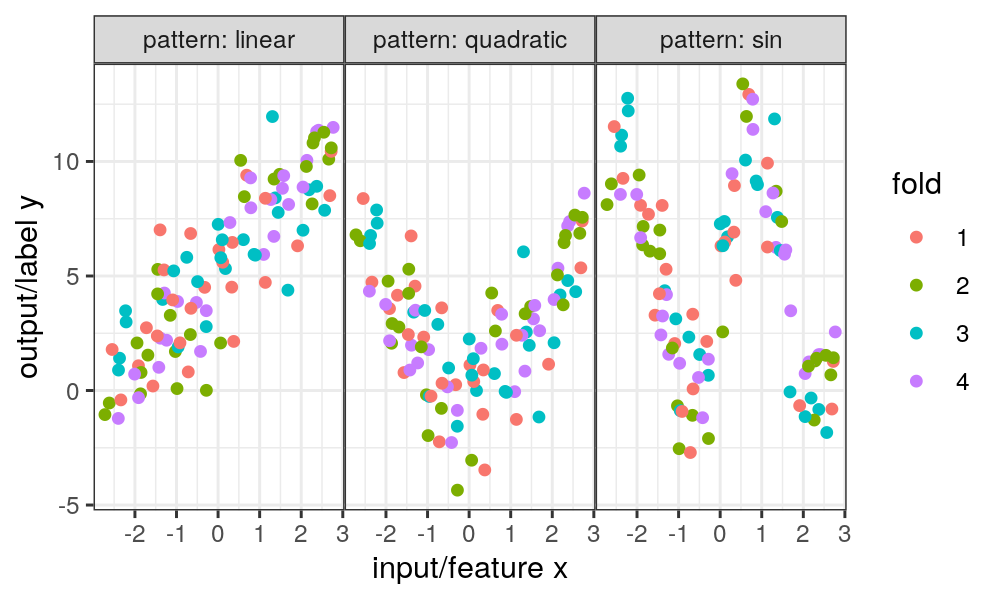
\includegraphics[width=\textwidth]{figure-overfitting-data-folds}

  Randomly assign each observation a fold ID from 1 to 4.
  
\end{frame}

\begin{frame}
  \frametitle{Illustration of subtrain/validation split}
  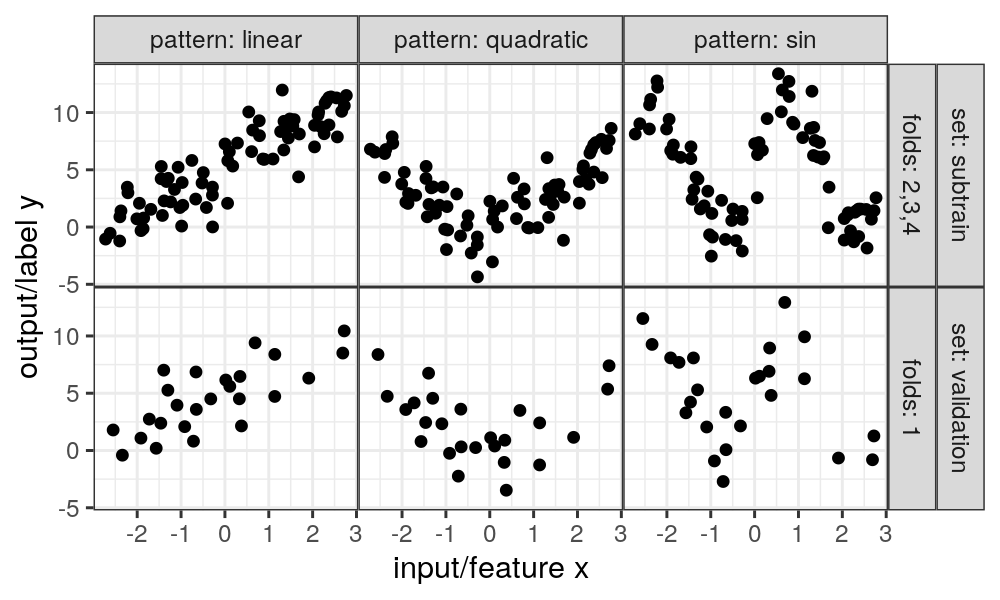
\includegraphics[width=\textwidth]{figure-overfitting-data-sets}

  \begin{itemize}
  \item For validation fold 1, all observations with that fold ID are
    considered the validation set.
  \item All other observations are considered the subtrain set.
  \end{itemize}
\end{frame}

\begin{frame}[fragile]
  \frametitle{CSV data tables for machine learning}
  \begin{itemize}
  \item One row for each observation.
  \item One column for the output/label/y (in regression the label is a real
    number, in classification the label is a class/category).
  \item The other columns should be inputs/features/X that will be used
    to predict the corresponding output/label/y.
  \end{itemize}

  Example:
  \url{https://raw.githubusercontent.com/tdhock/2020-yiqi-summer-school/master/data_linear.csv}

\begin{verbatim}
               x            y
  1: -1.40694802  0.933196336
  2: -0.76725660  3.832773444
  3:  0.43712018  4.202983135
  4:  2.44924674 13.089055084
...
\end{verbatim}
\end{frame}

\begin{frame}[fragile]
  \frametitle{Result of reading CSV data into R}
  Result is:

\begin{verbatim}
> sim.data
     pattern          x          y fold
  1:  linear -1.4069480  0.9331963    4
  2:  linear -0.7672566  3.8327734    3
  3:  linear  0.4371202  4.2029831    1
  4:  linear  2.4492467 13.0890551    2
  5:  linear -1.7899084  2.0791987    3
 ---                                   
296:     sin  1.7838530  4.0502991    1
297:     sin -0.2683533 -0.1097264    1
298:     sin -0.5394955 -0.5539398    1
299:     sin  1.8652215 -0.2262517    4
300:     sin  0.6295997  8.8124249    4
\end{verbatim}
  
\end{frame}

\begin{frame}[fragile]
  \frametitle{Assign each observation to subtrain/validation set}

\begin{verbatim}
validation.fold <- 1
sim.data[, set := ifelse(
  fold==validation.fold, "validation", "subtrain")]
> sim.data
     pattern          x          y fold        set
  1:  linear -1.4069480  0.9331963    4   subtrain
  2:  linear -0.7672566  3.8327734    3   subtrain
  3:  linear  0.4371202  4.2029831    1 validation
  4:  linear  2.4492467 13.0890551    2   subtrain
  5:  linear -1.7899084  2.0791987    3   subtrain
 ---                                              
296:     sin  1.7838530  4.0502991    1 validation
297:     sin -0.2683533 -0.1097264    1 validation
298:     sin -0.5394955 -0.5539398    1 validation
299:     sin  1.8652215 -0.2262517    4   subtrain
300:     sin  0.6295997  8.8124249    4   subtrain
\end{verbatim}
  
\end{frame}

\begin{frame}[fragile]
  \frametitle{Neural network with one hidden layer, 20 hidden units}

  Use for loops to fit different neural network models for each data
  set and number of iterations. 

\begin{verbatim}
maxit.values <- 10^seq(0, 4)
pattern.values <- c("linear", "quadratic", "sin")
for(i in maxit.values)for(p in pattern.values){
  pattern.data <- sim.data[pattern==p]
  fit <- nnet::nnet(
    y ~ x,
    pattern.data[set=="subtrain"],
    size=20,     #hidden units
    linout=TRUE, #for regression
    maxit=i)     #max number of iterations
...
\end{verbatim}

\end{frame}

\begin{frame}
  \frametitle{Neural network prediction function}
\begin{equation*}
  f(\mathbf x) = f_L[\cdots f_1[\mathbf x] ].
\end{equation*}
For the nnet code, we have:
\begin{eqnarray*}
  f_1(t) &=& A_1( \mathbf W_1^\intercal t ), \\
  f_2(t) &=& A_2( \mathbf W_2^\intercal t ), \\
  f(x) &=& f_2[ f_1(x) ] = A_2[ \mathbf W_2^\intercal A_1( \mathbf W_1^\intercal x ) ].
\end{eqnarray*}
The hyper-parameters are fixed prior to learning:
\begin{itemize}
\item Number of layers $L=2$.
\item Activation functions $A_1$=sigmoid, $A_2$=identity.
\item Number of units in the hidden layer $u_1=20$.
\item No sparsity in the weight matrices (fully connected).
\end{itemize}
The weight matrices $\mathbf W_1,\mathbf W_2$ are learned using
gradient descent.
\begin{itemize}
\item ``Full gradient'' method is used, so in each \textbf{epoch}
  there is 1 iteration/update to the weights that is based on the
  gradient summed over all subtrain data.
\end{itemize}

\end{frame}


\begin{frame}
  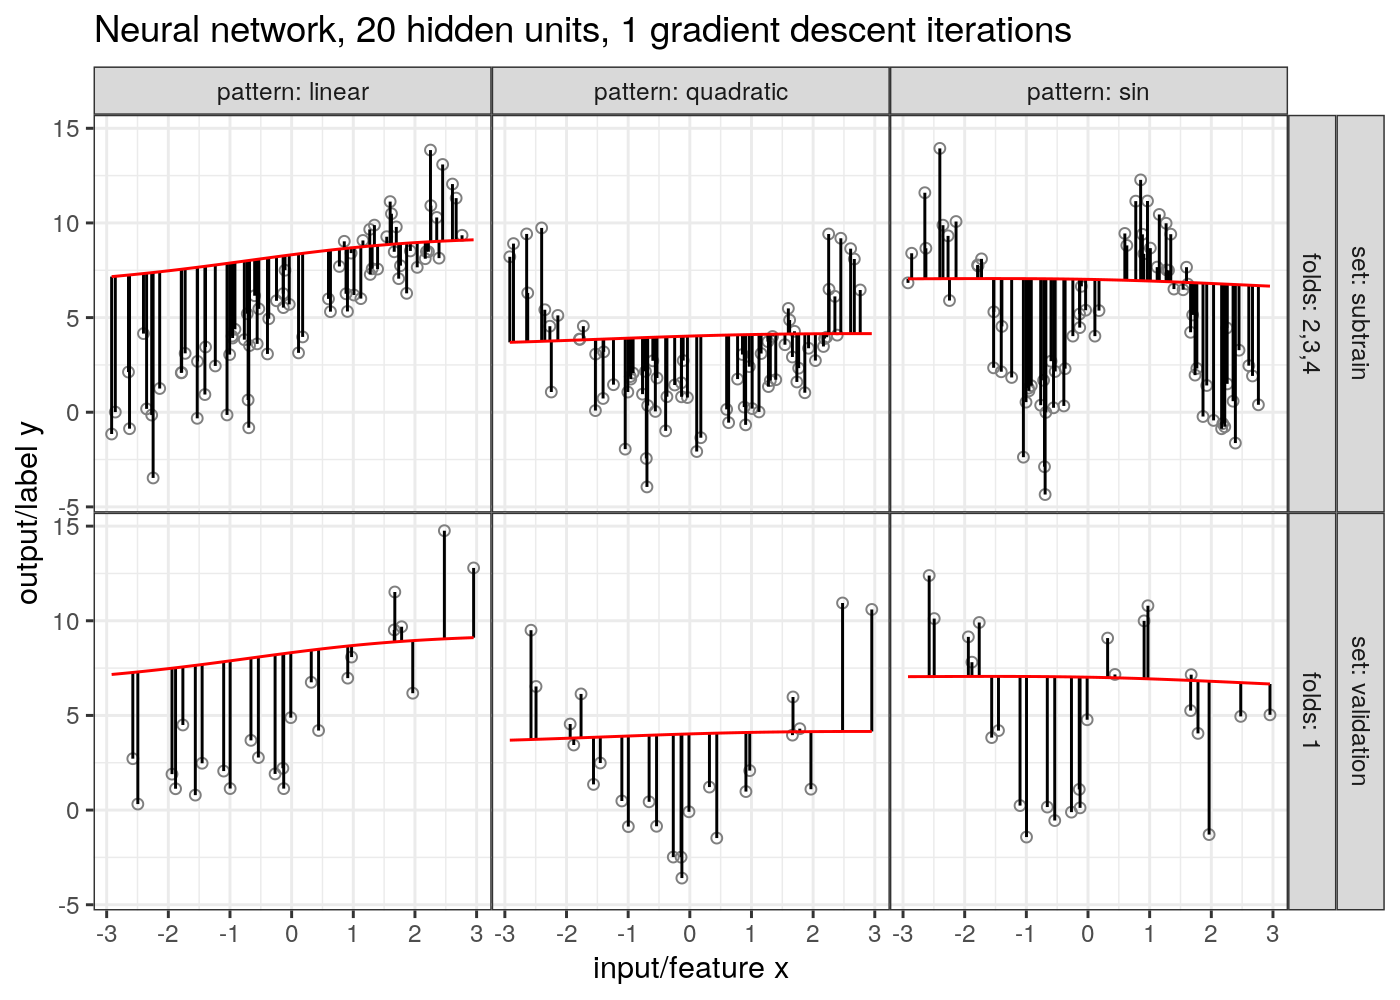
\includegraphics[width=\textwidth]{figure-overfitting-pred-units=20-maxit=1.png}
\end{frame}


\begin{frame}
  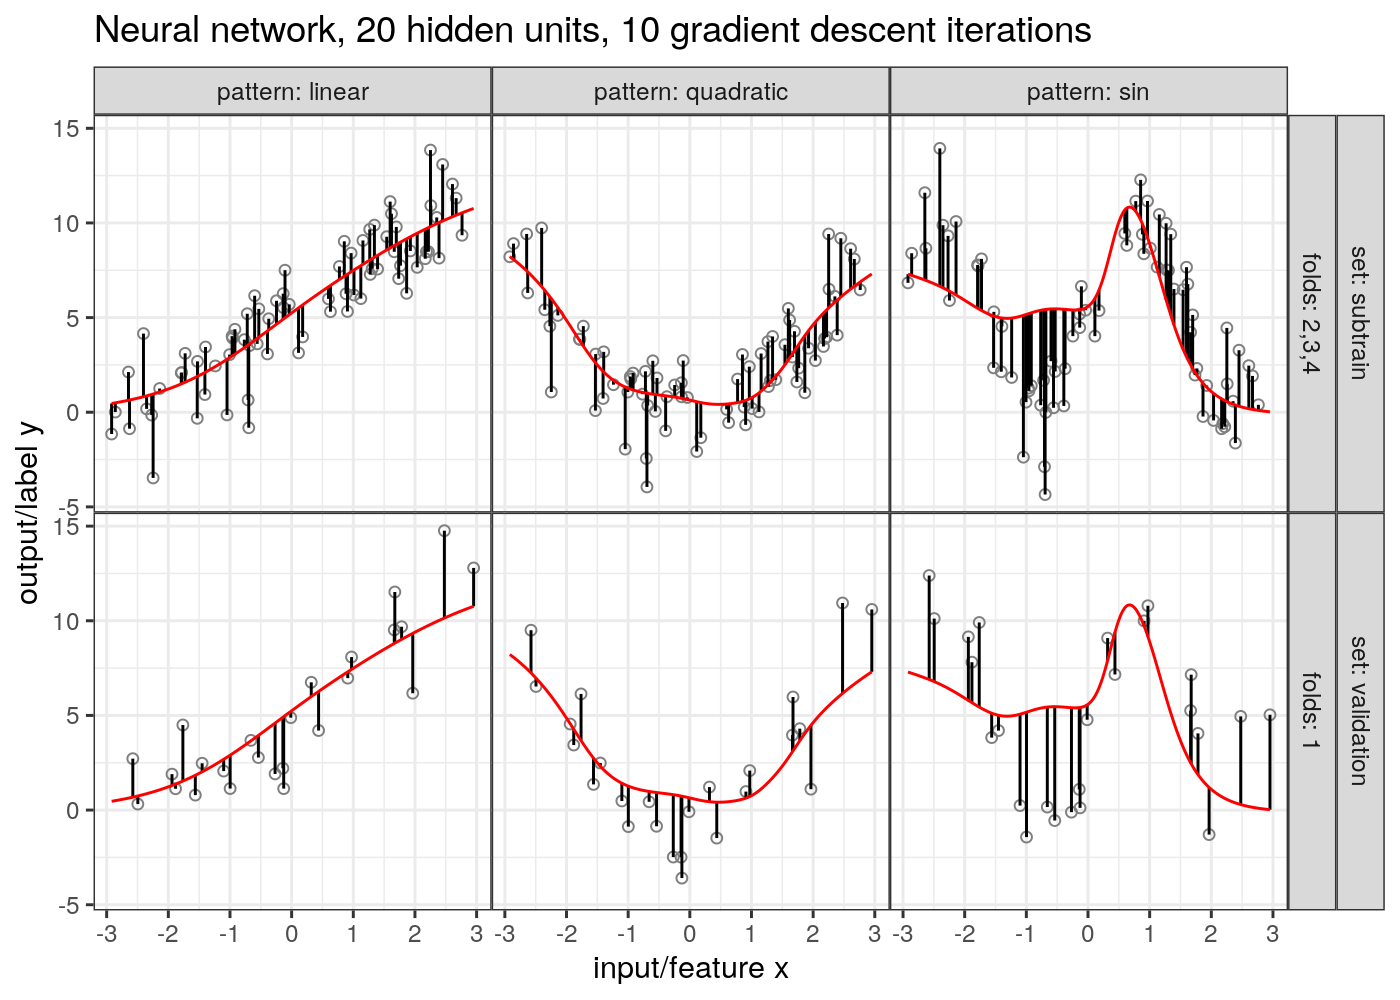
\includegraphics[width=\textwidth]{figure-overfitting-pred-units=20-maxit=10.png}
\end{frame}


\begin{frame}
  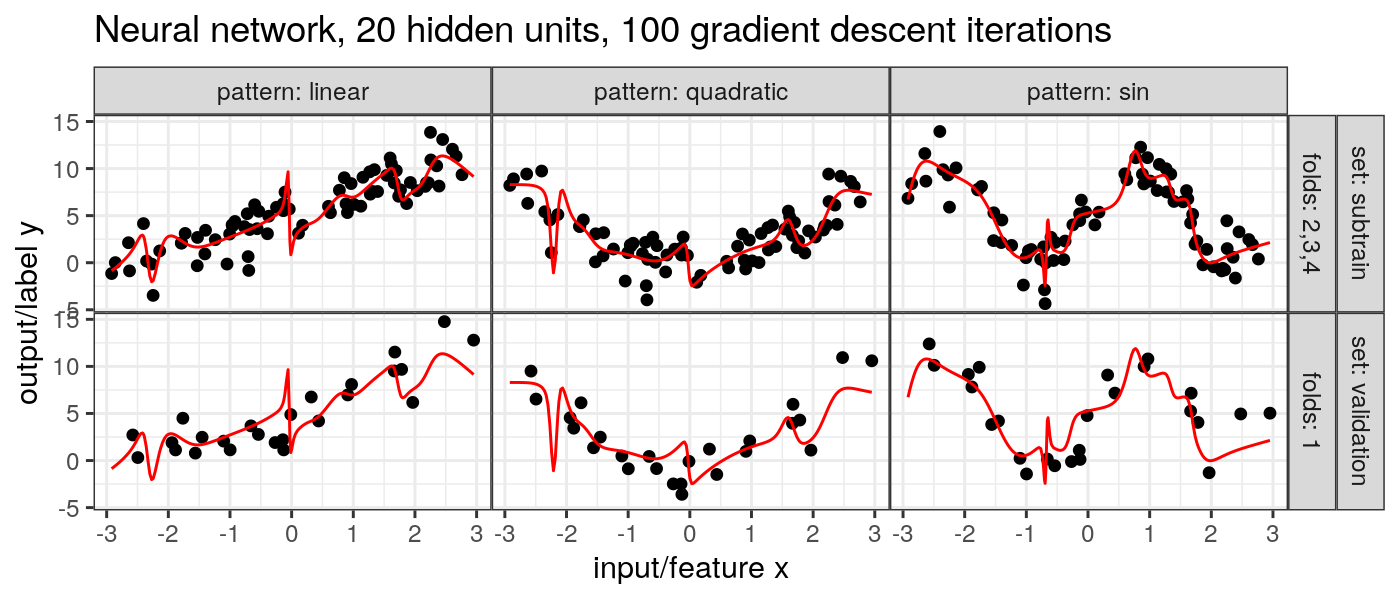
\includegraphics[width=\textwidth]{figure-overfitting-pred-units=20-maxit=100.png}
\end{frame}


\begin{frame}
  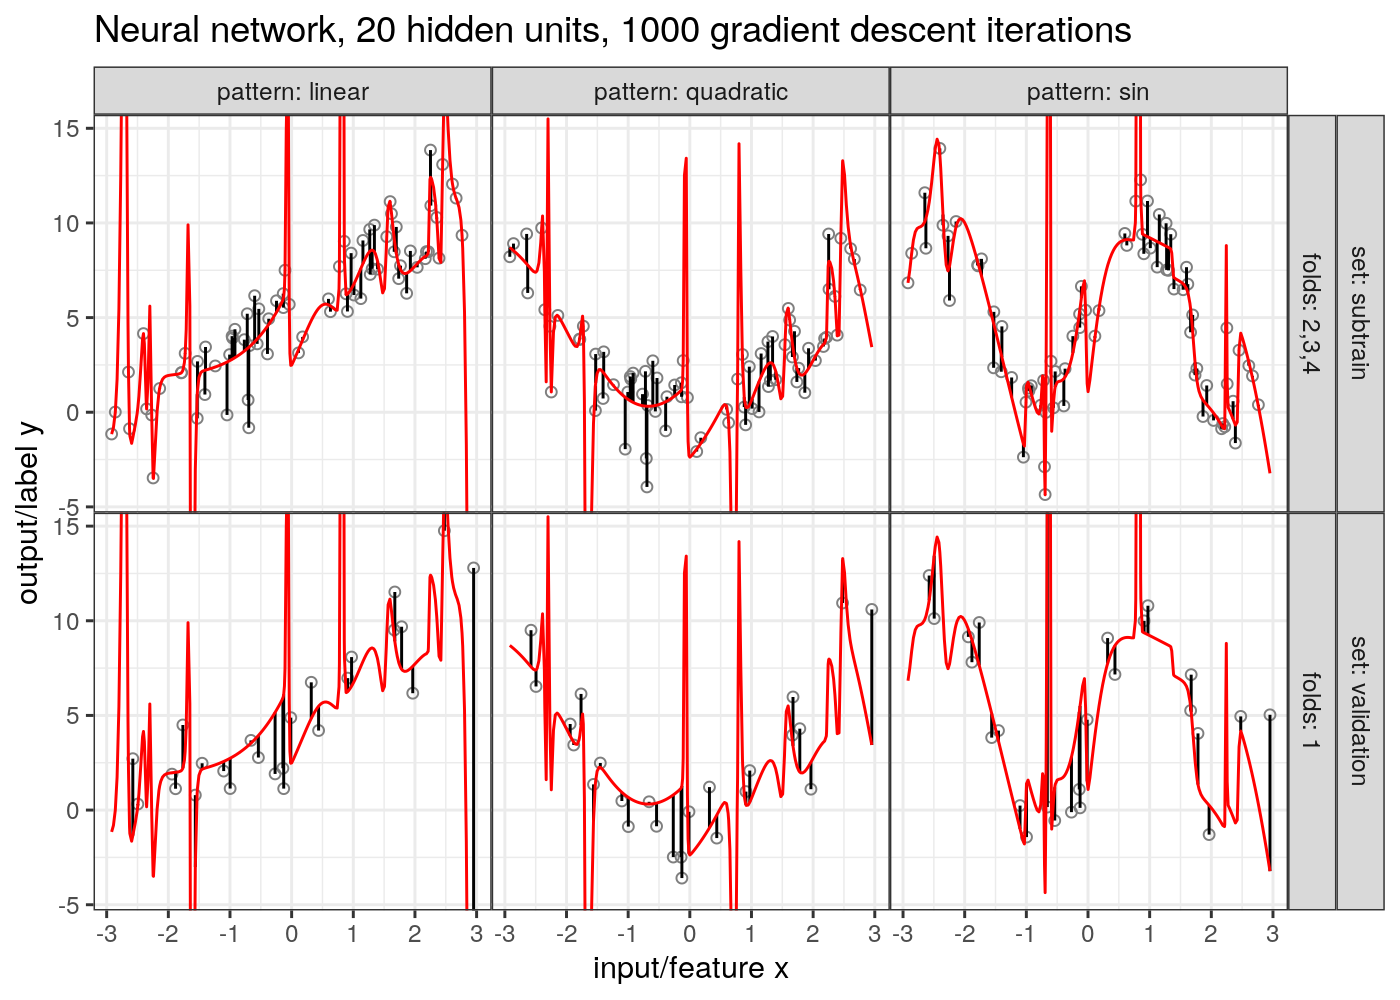
\includegraphics[width=\textwidth]{figure-overfitting-pred-units=20-maxit=1000.png}
\end{frame}


\begin{frame}
  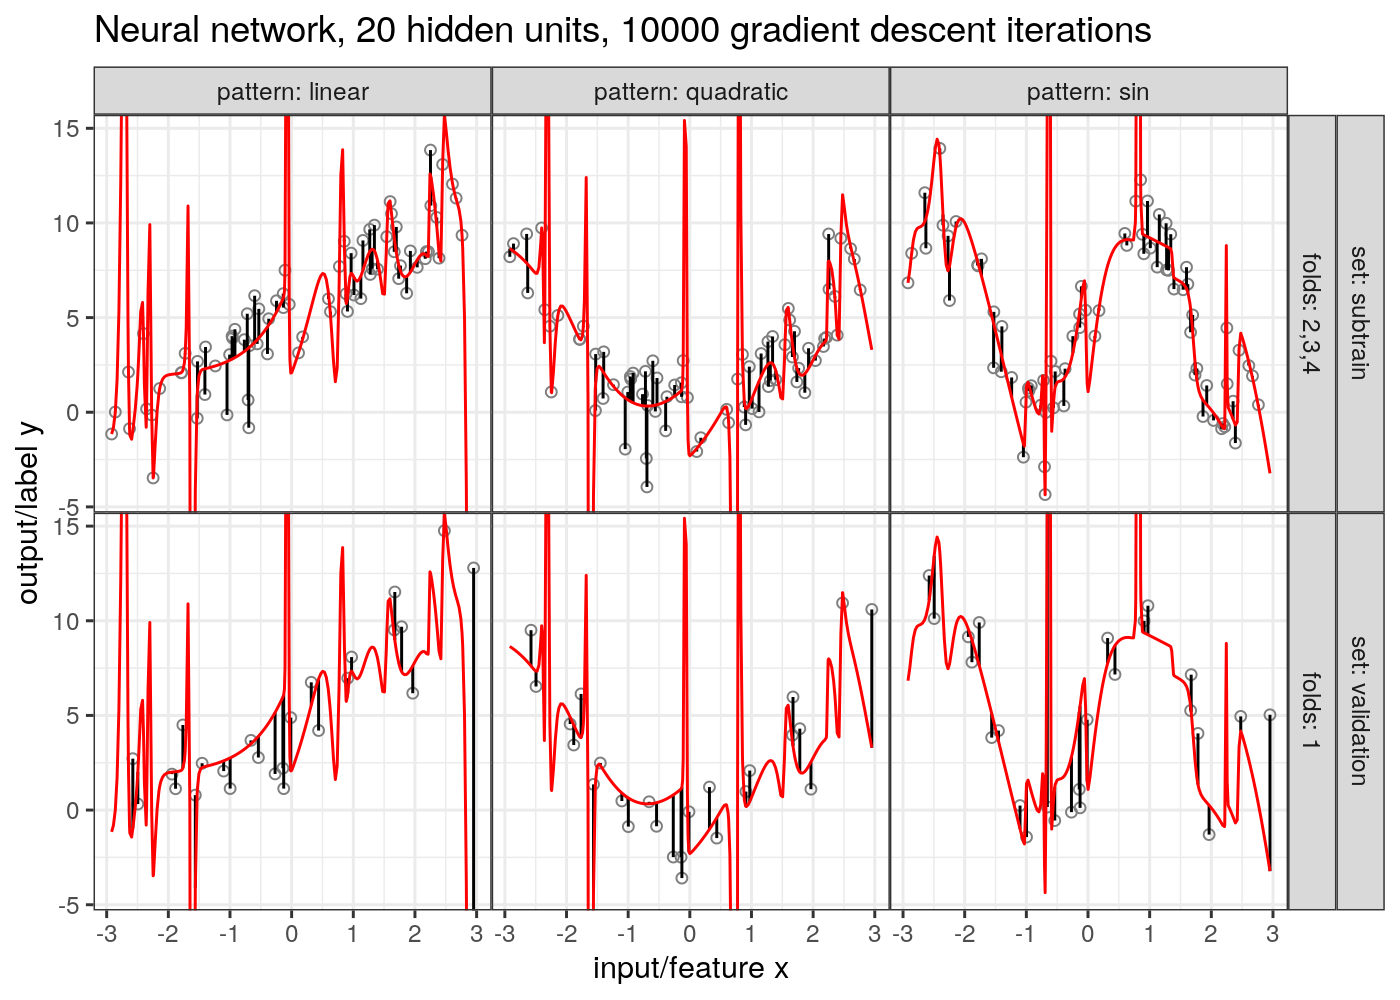
\includegraphics[width=\textwidth]{figure-overfitting-pred-units=20-maxit=10000.png}
\end{frame}


\begin{frame}
  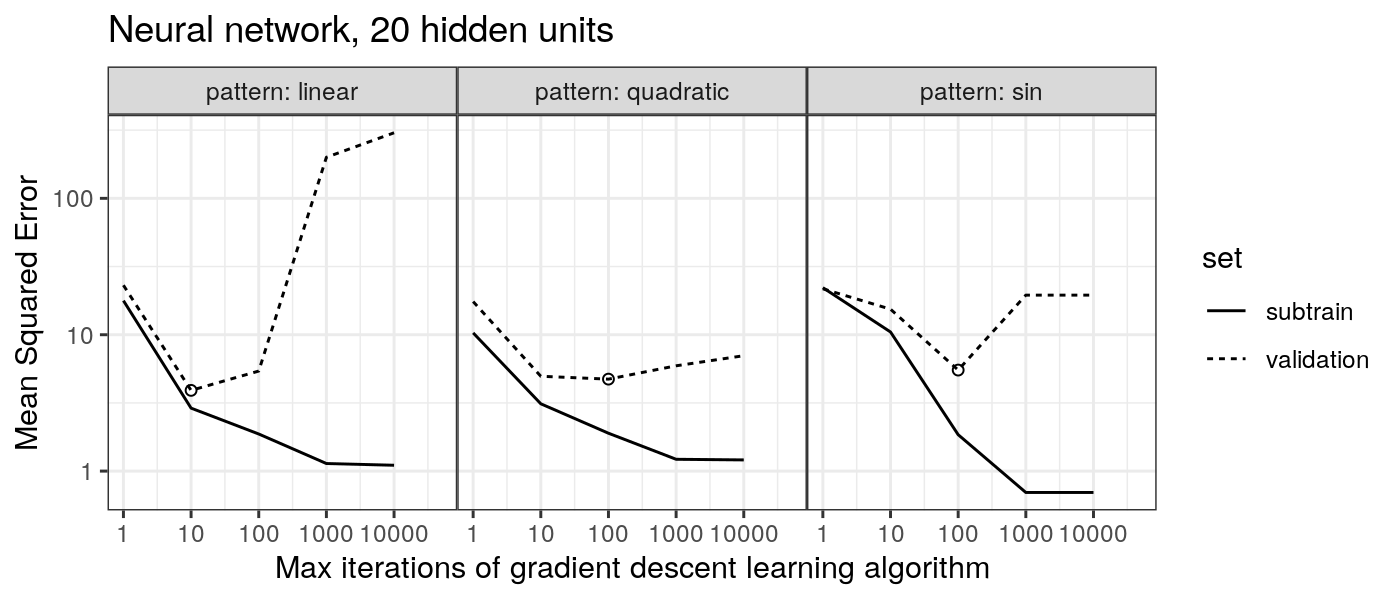
\includegraphics[width=\textwidth]{figure-overfitting-data-loss-20.png}
\end{frame}




\begin{frame}
  \centering
  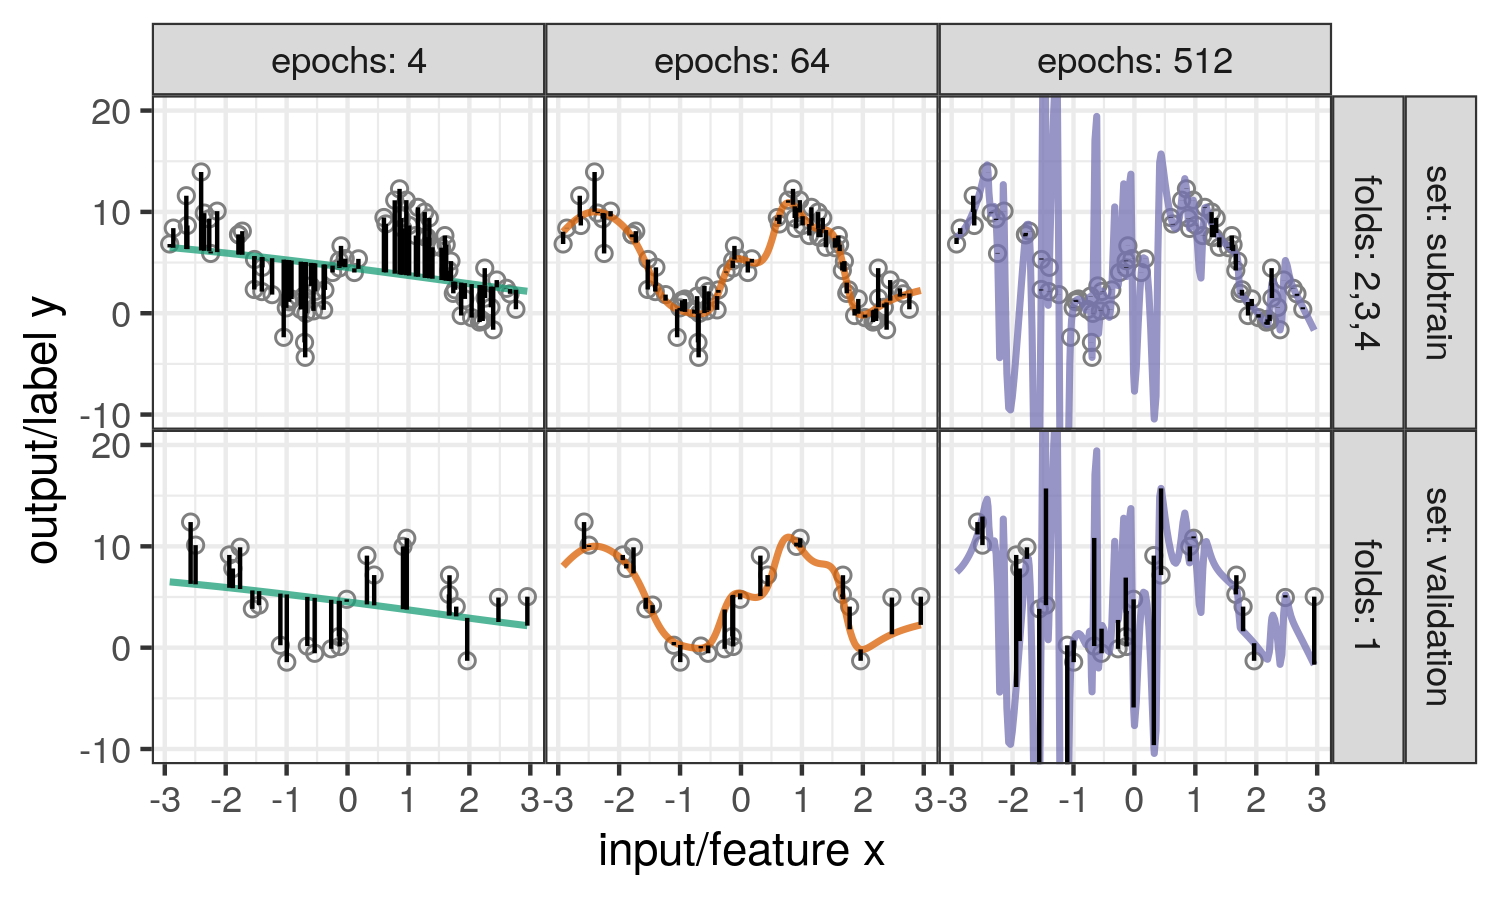
\includegraphics[height=0.5\textheight]{figure-overfitting-paper}
  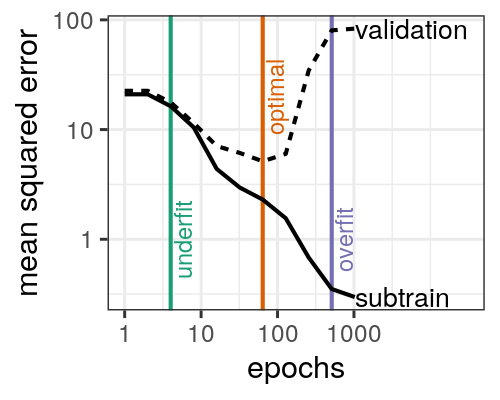
\includegraphics[height=0.45\textheight]{figure-overfitting-paper-loss}   
\end{frame}

\begin{frame}
  \frametitle{Summary of how to avoid overfitting}
  \begin{itemize}
  \item Happens when subtrain error/loss decreases but validation error
    increases (as a function of some hyper-parameter)
  \item Here the hyper-parameter is the number of iterations of
    gradient descent, and overfitting starts after a certain number of
    iterations.
  \item To maximize prediction accuracy you need to choose a
    hyper-parameter with minimal validation error/loss.
  \item This optimal hyper-parameter will depend on the data set.
  \item To get optimal prediction accuracy in any machine learning
    analysis, you always need to do this, because you never know the
    best hyper-parameters in advance.
  \end{itemize}
\end{frame}

\section{Example 2: classifying images of digits
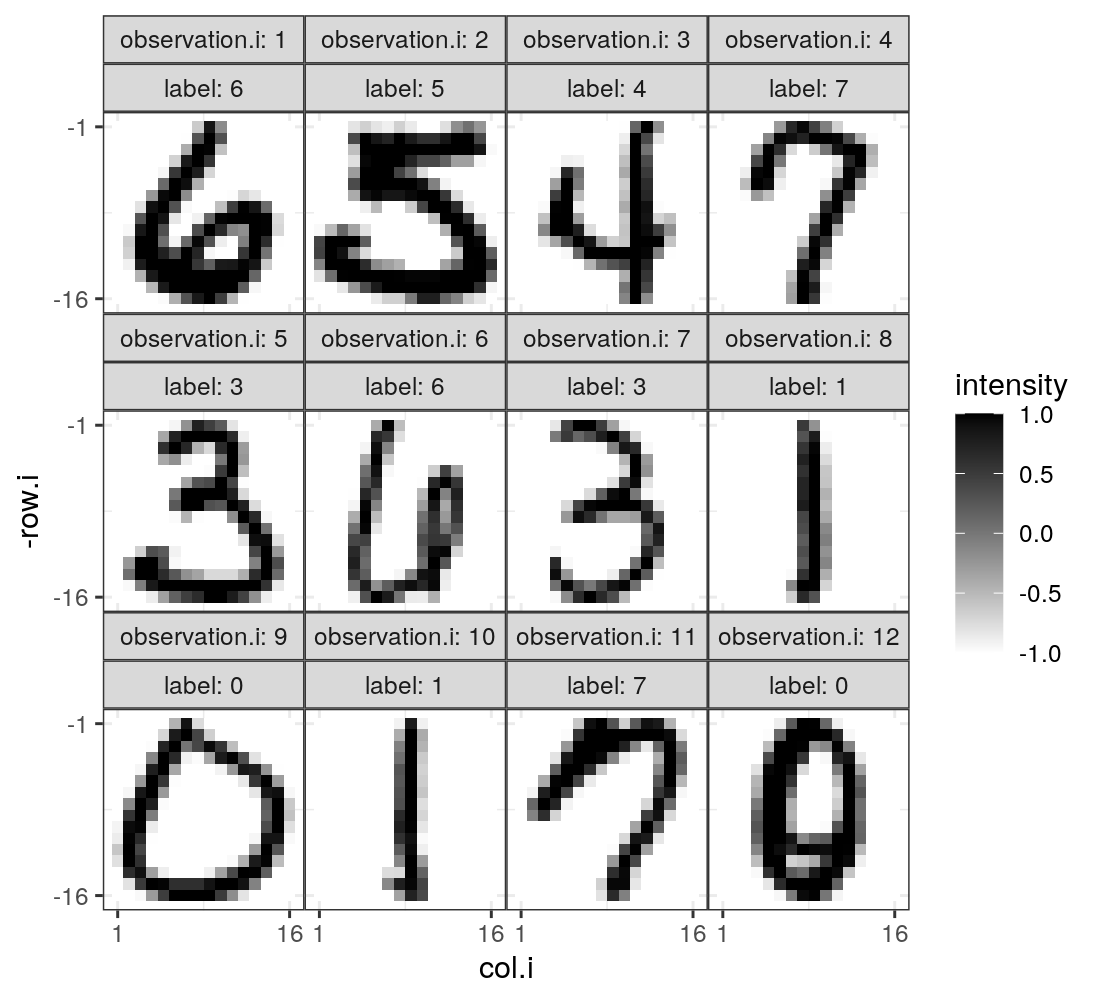
\includegraphics[height=2cm]{figure-validation-loss-digits}}

\begin{frame}
  \frametitle{Image classification}
  \begin{itemize}
  \item One of the most popular/successful applications of machine
    learning.
  \item Input: image file $x\in\mathbb R^{h\times w\times c}$ where
    $h$ is the height in pixels, $w$ is the width, $c$ is the number
    of channels, e.g. RGB image $c=3$ channels.
  \item In this tutorial we use images with $h=w=16$ pixels and $c=1$
    channel (grayscale, smaller values are darker).
  \item Output: class/category $y$ (from a finite set).
  \item In this tutorial there are ten image classes $y\in\{0, 1, \dots, 9\}$, one for each
    digit.
  \item Want to learn $f$ such that
    $f(
\includegraphics[height=1cm]{mnist-0})=0$,
    $f(
\includegraphics[height=1cm]{mnist-1})=1$, etc.
  \item Code for figures in this section:
    \url{https://github.com/tdhock/2020-yiqi-summer-school/blob/master/figure-validation-loss.R}
  \end{itemize}
\end{frame}

\begin{frame}
  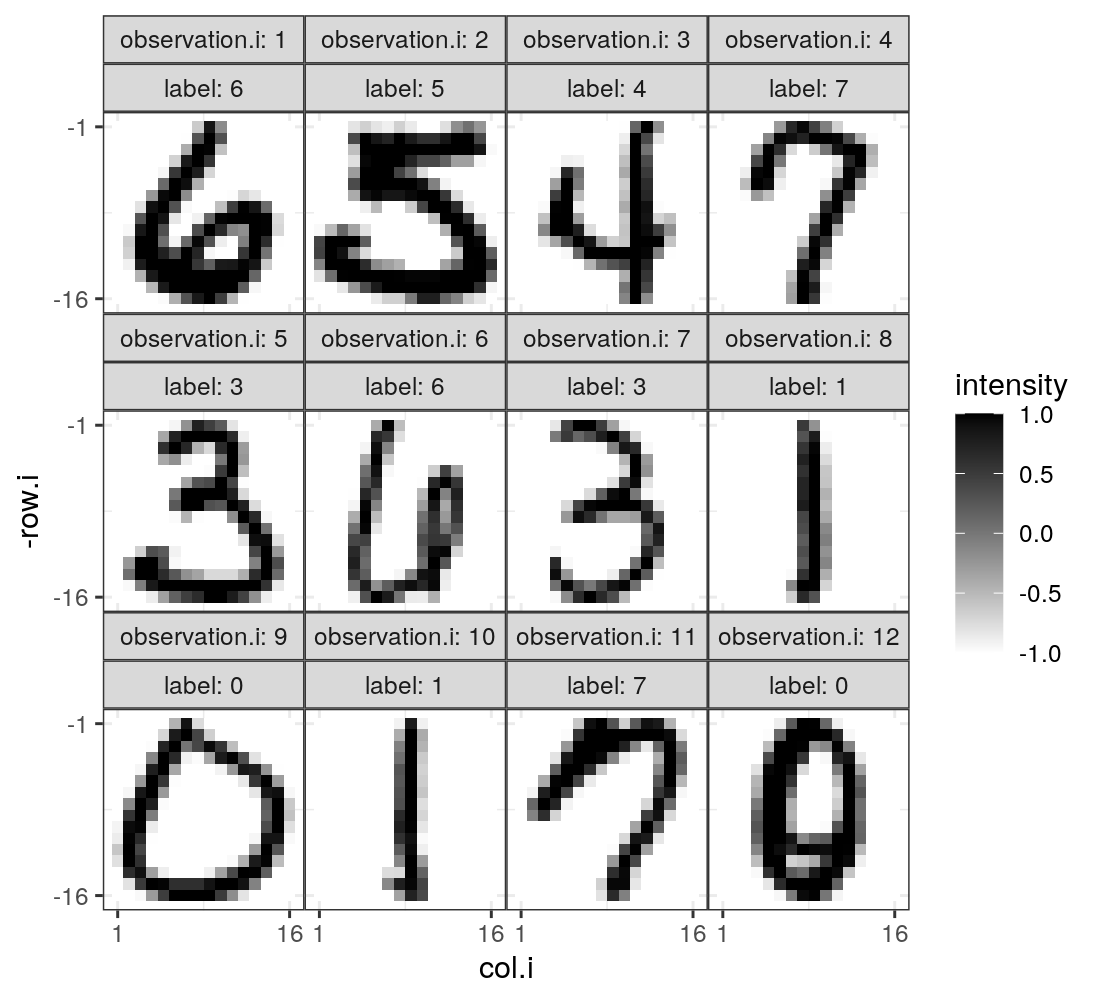
\includegraphics[height=\textheight]{figure-validation-loss-digits}
\end{frame}

\begin{frame}[fragile]
  \frametitle{Representation of digits in CSV}

  \begin{itemize}
  \item Each image/observation is one row.
  \item First column is output/label/class to predict.
  \item Other 256 columns are inputs/features (pixel intensity
    values).
  \end{itemize}
 Data from {\scriptsize \url{https://web.stanford.edu/~hastie/ElemStatLearn/datasets/zip.train.gz}}

\begin{verbatim}
 1:  6 -1 -1  ... -1.000 -1.000   -1
 2:  5 -1 -1  ... -0.671 -0.828   -1
 3:  4 -1 -1  ... -1.000 -1.000   -1
 4:  7 -1 -1  ... -1.000 -1.000   -1
 5:  3 -1 -1  ... -0.883 -1.000   -1
 6:  6 -1 -1  ... -1.000 -1.000   -1
...
\end{verbatim}
  
\end{frame}

\begin{frame}[fragile]
  \frametitle{Converting label column to matrix for neural network}

  This is a ``one hot'' encoding of the class labels.  
  
\begin{verbatim}
zip.dt <- data.table::fread("zip.gz")
zip.y.mat <- keras::to_categorical(zip.dt$V1)

      0 1 2 3 4 5 6 7 8 9
 [1,] 0 0 0 0 0 0 1 0 0 0
 [2,] 0 0 0 0 0 1 0 0 0 0
 [3,] 0 0 0 0 1 0 0 0 0 0
 [4,] 0 0 0 0 0 0 0 1 0 0
 [5,] 0 0 0 1 0 0 0 0 0 0
 [6,] 0 0 0 0 0 0 1 0 0 0
...
\end{verbatim}


\end{frame}

\begin{frame}[fragile]
  \frametitle{Converting inputs to tensor (multi-dim array) for neural network}
Use array function with all columns except first as data.  
\begin{verbatim}
zip.size <- 16
zip.X.array <- array(
  data = unlist(zip.dt[1:nrow(zip.dt),-1]),
  dim = c(nrow(zip.dt), zip.size, zip.size, 1))
\end{verbatim}
Need to specify dimensions of array:
\begin{itemize}
\item Observations: same as the number of rows in the CSV table.
\item Pixels wide: 16.
\item Pixels high: 16.
\item Channels: 1 (greyscale image).
\end{itemize}

\end{frame}

\begin{frame}[fragile]
  \frametitle{Linear model R code}

\begin{verbatim}
library(keras)
linear.model <- keras::keras_model_sequential() %>%
  keras::layer_flatten(
    input_shape = c(16, 16, 1)) %>%
  keras::layer_dense(
    units = 10,
    activation = 'softmax')
\end{verbatim}

  \begin{itemize}
  \item First layer must specify shape of inputs (here 16x16x1).
  \item \texttt{layer\_flatten} converts any shape to a single dimension
    of units (here 256).
  \item \texttt{layer\_dense} uses all units in the previous layer to
    predict each unit in the layer.
  \item \texttt{units=10} because there are ten possible classes for an output.
  \item \texttt{activation='softmax'} is required for the last/output layer in
    multi-class classification problems.
  \end{itemize}

\end{frame}

\begin{frame}[fragile]
\frametitle{Keras model compilation}
\begin{verbatim}
linear.model %>% keras::compile(
  loss = keras::loss_categorical_crossentropy,
  optimizer = keras::optimizer_adadelta(),
  metrics = c('accuracy')
)
\end{verbatim}
In \texttt{compile} you can specify
\begin{itemize}
\item a \texttt{loss} function, which is directly optimized/minimized
  in each iteration of the gradient descent learning algorithm. 
  \url{https://keras.io/api/losses/} 
\item an \texttt{optimizer}, which is the version of gradient descent
  learning algorithm to use. 
  \url{https://keras.io/api/optimizers/} 
\item an evaluation \texttt{metric} to monitor, not directly optimized
  via gradient descent, but usually more relevant/interpretable for
  the application (e.g. accuracy is the proportion of correctly
  predicted labels). \url{https://keras.io/api/metrics/} 
\end{itemize}
\end{frame}
 
\begin{frame}[fragile]
\frametitle{Keras model fitting}
\begin{verbatim}
linear.model %>% keras::fit(
  zip.X.array, zip.y.mat,
  epochs = 50,
  validation_split = 0.2
)
\end{verbatim}
In \texttt{fit} you can specify
\begin{itemize}
\item Train data inputs \texttt{zip.X.array} and outputs
  \texttt{zip.y.mat} (required).
\item Number of full passes of gradient descent through the subtrain
  data (\texttt{epochs}). In each epoch the gradient with respect to
  each subtrain observation is computed once.
\item \texttt{validation\_split=0.2} which means to use 80\% subtrain
  (used for gradient descent parameter updates), 20\% validation (used
  for hyper-parameter selection). 
\end{itemize}
\end{frame}
 
\begin{frame}
  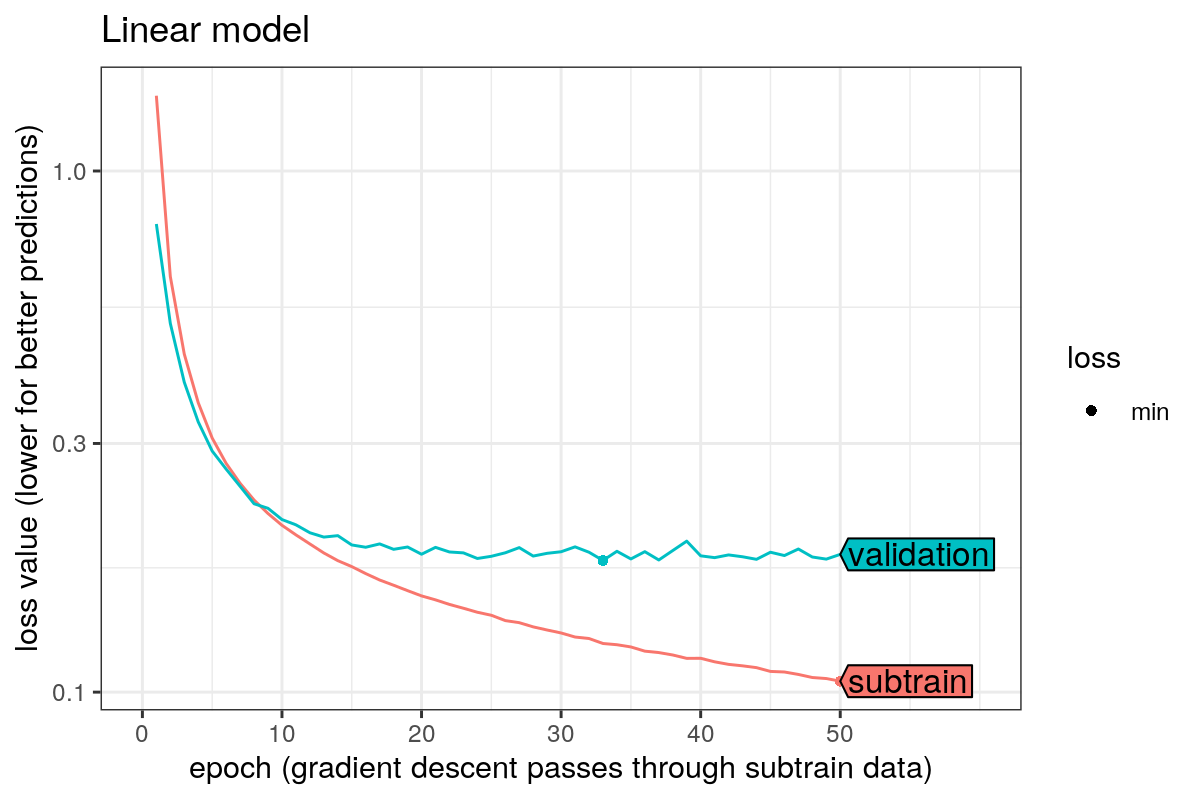
\includegraphics[width=\textwidth]{figure-validation-loss-linear}
\end{frame}
 
\begin{frame}[fragile]
  \frametitle{Sparse (convolutional) model R code}

\begin{verbatim}
library(keras)
conv.model <- keras_model_sequential() %>%
  layer_conv_2d(
    input_shape = dim(zip.X.array)[-1],
    filters = 20,
    kernel_size = c(3,3),
    activation = 'relu') %>% 
  layer_max_pooling_2d(pool_size = c(2, 2)) %>%
  layer_flatten() %>%
  layer_dense(units = 100, activation = 'relu') %>% 
  layer_dense(
    units = ncol(zip.y.mat), 
    activation = 'softmax')
\end{verbatim}

  \begin{itemize}
  \item Sparse: few inputs are used to predict each unit in
    \texttt{layer\_conv\_2d}.
  \item Exploits structure of image data to make learning
    easier/faster.
  \end{itemize}

\end{frame}
 
\begin{frame}
  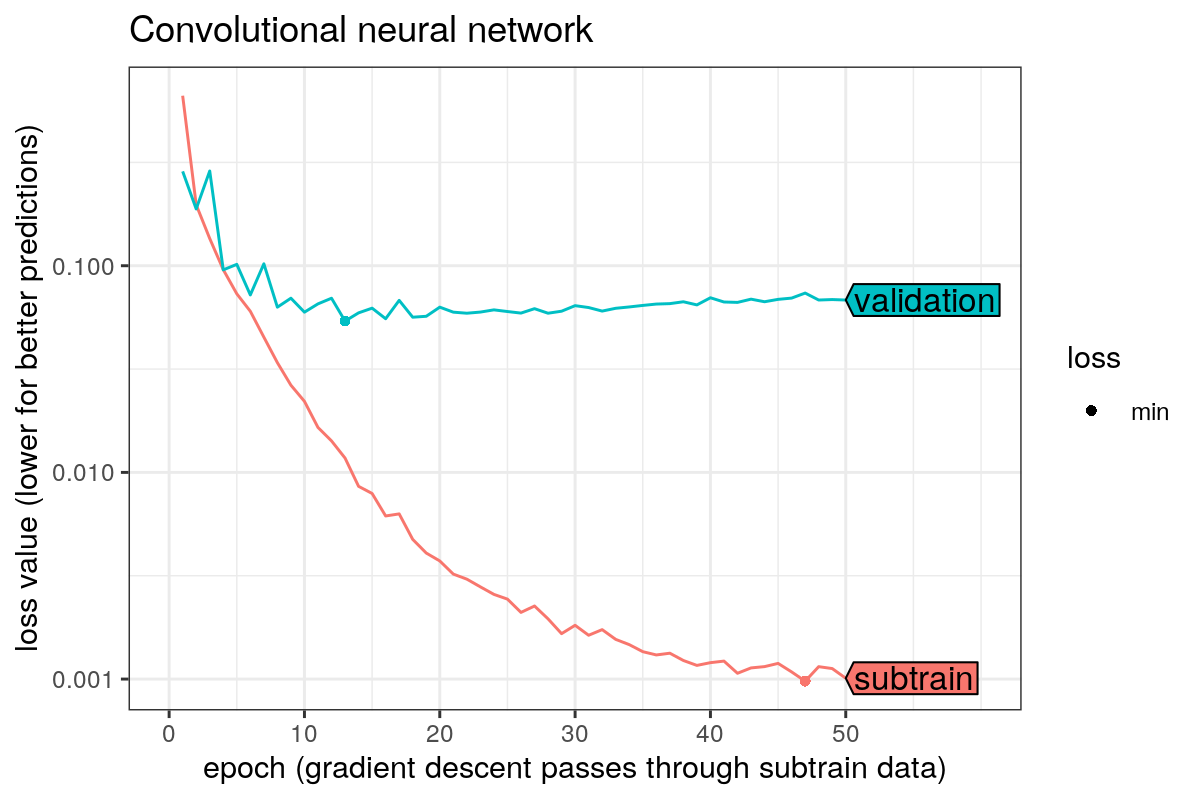
\includegraphics[width=\textwidth]{figure-validation-loss-conv}
\end{frame}
 
\begin{frame}[fragile]
  \frametitle{Dense (fully connected) neural network R code}

\begin{verbatim}
library(keras)
dense.model <- keras_model_sequential() %>%
  layer_flatten(
    input_shape = dim(zip.X.array)[-1]) %>%
  layer_dense(units = 100, activation = 'relu') %>% 
  layer_dense(units = 100, activation = 'relu') %>% 
  layer_dense(units = 100, activation = 'relu') %>% 
  layer_dense(units = 100, activation = 'relu') %>%
  layer_dense(units = 100, activation = 'relu') %>%
  layer_dense(units = 100, activation = 'relu') %>% 
  layer_dense(units = 100, activation = 'relu') %>%   
  layer_dense(units = 100, activation = 'relu') %>% 
  layer_dense(
    units = ncol(zip.y.mat), 
    activation = 'softmax')
\end{verbatim}

\end{frame}
 
\begin{frame}
  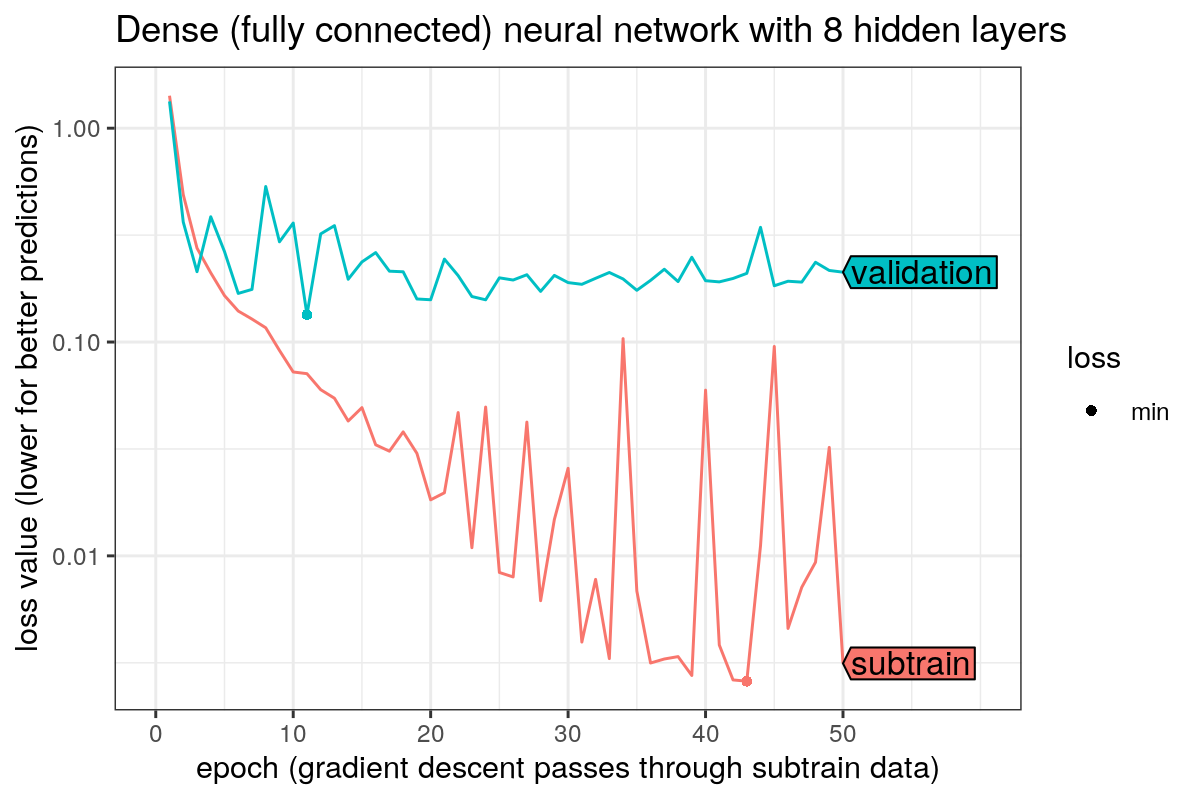
\includegraphics[width=\textwidth]{figure-validation-loss-dense}
\end{frame}
 
\begin{frame}
  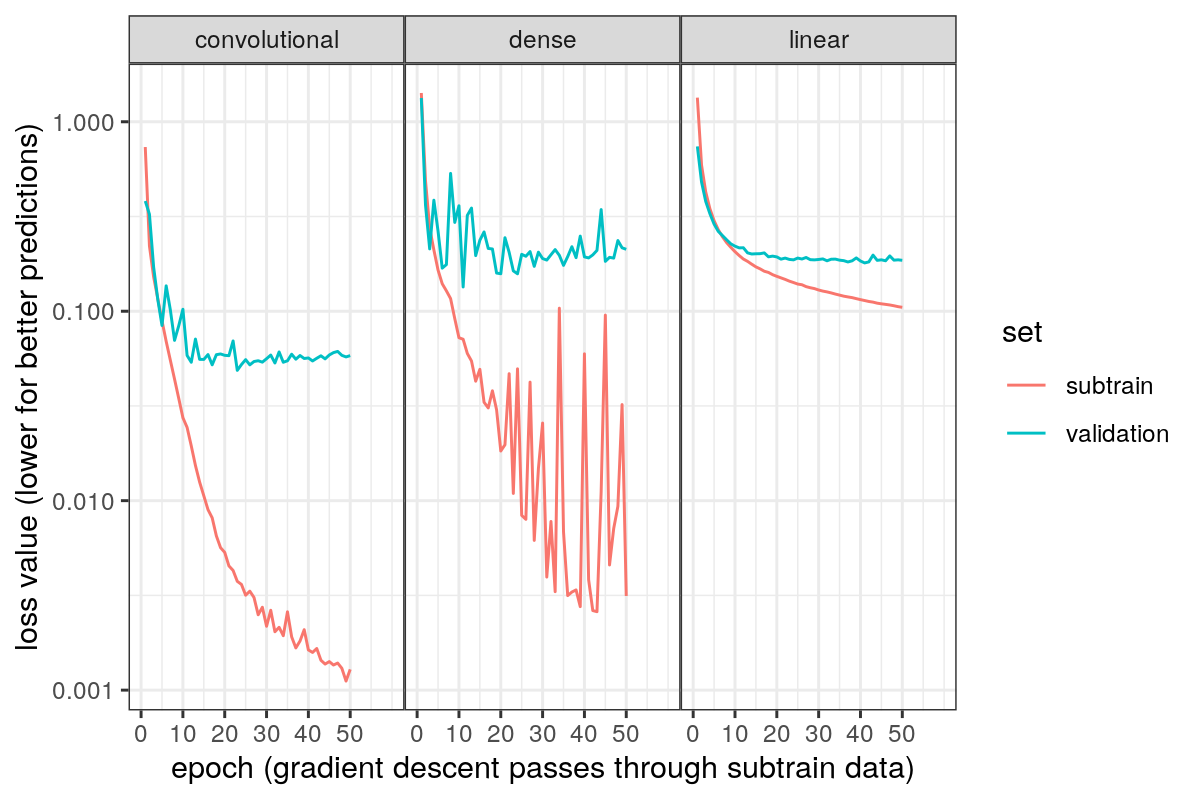
\includegraphics[width=\textwidth]{figure-validation-loss-three}
\end{frame}

\begin{frame}
  \frametitle{K-fold cross-validation for model evaluation}
  Is convolutional more accurate on unseen test data?
  
  \includegraphics[width=\textwidth]{drawing-cross-validation}
  
  \begin{itemize}
  \item Randomly assign a fold ID from 1 to K to each observation.
  \item Hold out the observations with the Split ID as test set.
  \item Use the other observations as the train set.
  \item Run learning algorithm on train set (including hyper-parmeter
    selection), outputs learned function (f1-f3).
  \item Finally compute and plot the prediction accuracy (A1-A3) with
    respect to the held-out test set.
  \end{itemize}
\end{frame}


 
\begin{frame}
  \frametitle{Accuracy rates for each test fold}
  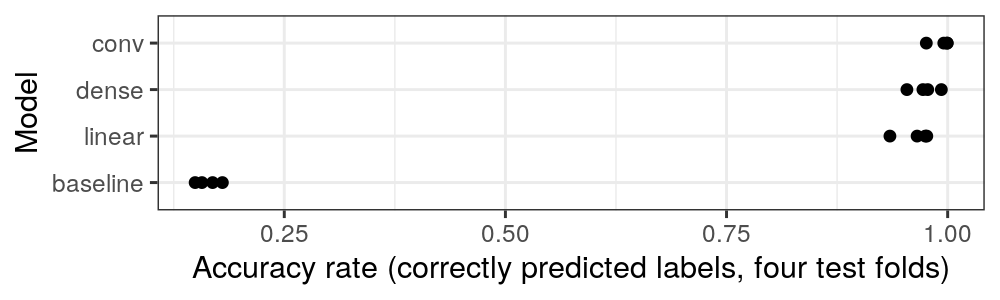
\includegraphics[width=\textwidth]{figure-test-accuracy-baseline}

  \begin{itemize}
  \item Always a good idea to compare with the trivial/featureless baseline model which always
    predicts the most frequent class in the train set. (ignoring all
    inputs/features) 
  \item Here we see that the featureless baseline is much less accurate than the
    three learned models, which are clearly learning something non-trivial.
  \item Code for test accuracy figures:
    \url{https://github.com/tdhock/2020-yiqi-summer-school/blob/master/figure-test-accuracy.R}
  \end{itemize}
\end{frame}
 
\begin{frame}
  \frametitle{Zoom to learned models}
  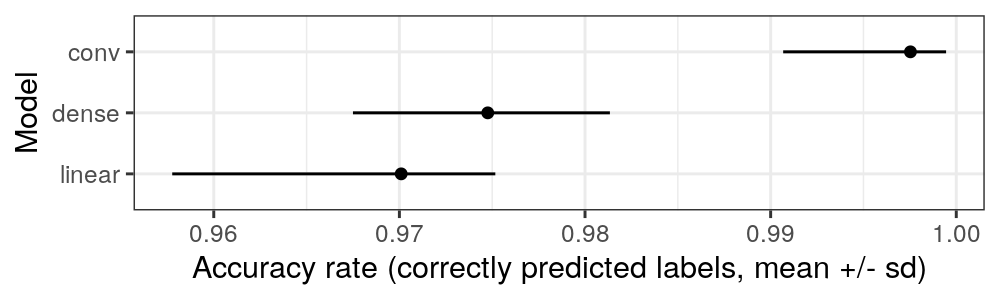
\includegraphics[width=\textwidth]{figure-test-accuracy}
  \begin{itemize}
  \item Dense neural network slightly more accurate
    than linear model, convolutional significantly more
    accurate than others.
  \item Conclusion: convolutional neural network should be preferred
    for most accurate predictions in these data.
  \item Maybe not the same conclusion in other data sets, with the
    same models. (always need to do cross-validation experiments to
    see which model is best in any given data set)
  \item Maybe other models/algorithms would be even more accurate in
    these data. (more/less layers, more/less units, completely
    different algorithm such as random forests, boosting, etc)
  \end{itemize}
\end{frame}

\section{Example 3: predicting earth system parameters 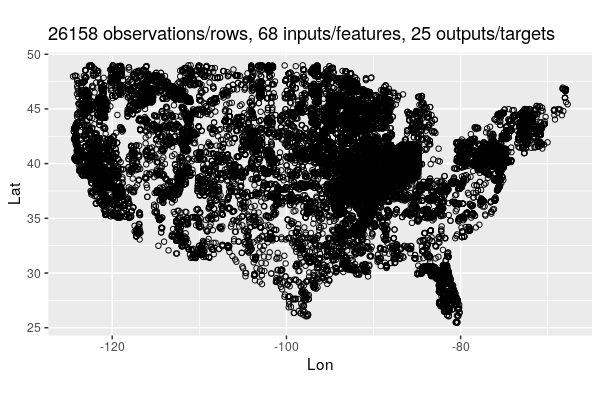
\includegraphics[height=2cm]{figure-proda-inputs}} 

\begin{frame}[fragile]
  \frametitle{Problem setting}
  Data from: F. Tao, Z. Zhou, Y. Huang, Q. Li, X. Lu, S. Ma, X. Huang,
  Y. Liang, G. Hugelius, L. Jiang, R. Doughty, Z. Ren, and
  Y. Luo. Deep learning optimizes data-driven representation of soil
  organic carbon in earth system model over the conterminous United
  States. Frontiers in Big Data, 3:17, 2020.

  \centering
  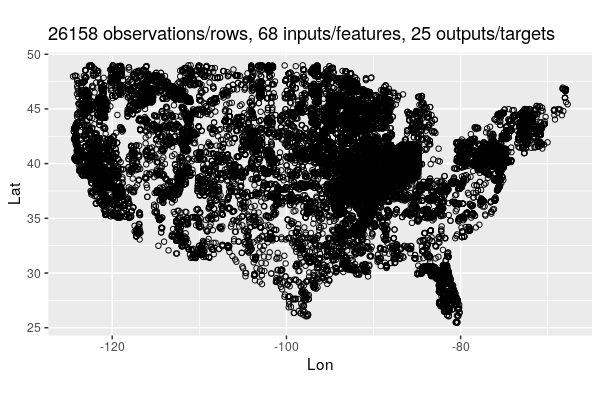
\includegraphics[width=0.7\textwidth]{figure-proda-inputs}

  Soil vertical profile data gathered at shown sites, and used to
  fit an earth system model.

\end{frame}

\begin{frame}[fragile]
  \frametitle{Inputs}
  Each site (row) has the following environmental features (columns):
\begin{verbatim}
        Lat       Lon Climate Soil_Type Veg_Cover ...
1: 47.24611 -111.0525       2        11        10
2: 47.68296 -111.2014       2        11        10
3: 45.35806 -116.8119       3        11        10
4: 46.73885 -102.7589       4        11        12
5: 47.65490 -111.5828       2        11        10
6: 48.49139 -109.8028       2        11        10
...
\end{verbatim}
  
\end{frame}

\begin{frame}[fragile]
  \frametitle{Outputs}
  We have fit an earth system model, which has the following
  parameters (columns) at each site (rows):
\begin{verbatim}
          cryo    maxpsi     tau4s3     fs2s3
[1,] 0.5559403 0.4472416 0.04058302 0.4105497
[2,] 0.4982079 0.5201390 0.19487388 0.3721377
[3,] 0.4878875 0.4155263 0.30624590 0.4009429
[4,] 0.4976373 0.4327989 0.25603125 0.1208804
[5,] 0.4469068 0.4972995 0.41847923 0.1809647
[6,] 0.4836617 0.4874783 0.17804971 0.2925210
...
\end{verbatim}
  
\end{frame}

\begin{frame}
  \frametitle{Problem statement}
  To what extent can we predict the earth system model parameters at a
  new site, assuming we have the environmental features / inputs
  available?
  \begin{itemize}
  \item Cross-validation splits data into train and test sets.
  \item Neural network learning algorithm run on train set.
  \item Predictions and accuracy/loss computed on test set.
\end{itemize}

    \centering
    \includegraphics[width=\textwidth]{drawing-cross-validation}
    
  
  \end{frame}

  \begin{frame}[fragile]
    \frametitle{Neural network architecture taken from paper}
\begin{verbatim}
    keras_model_sequential() %>%
      layer_dense(
        units = 256, activation = 'relu',
        input_shape = ncol(keep.mat.list[["input"]])) %>%
      layer_dropout(0.3) %>%
      layer_dense(units = 512, activation = 'relu') %>%
      layer_dropout(0.5) %>%
      layer_dense(units = 512, activation = 'relu') %>%
      layer_dropout(0.5) %>%
      layer_dense(units = 256, activation = 'relu') %>%
      layer_dropout(0.3) %>%
      layer_dense(units = 1 OR 25) %>%
      compile(
        loss = loss_mean_squared_error,
        optimizer = optimizer_adadelta()
      )
\end{verbatim}
  \end{frame}

\begin{frame}
  \frametitle{Neural networks often more accurate than featureless baseline }
  \centering
  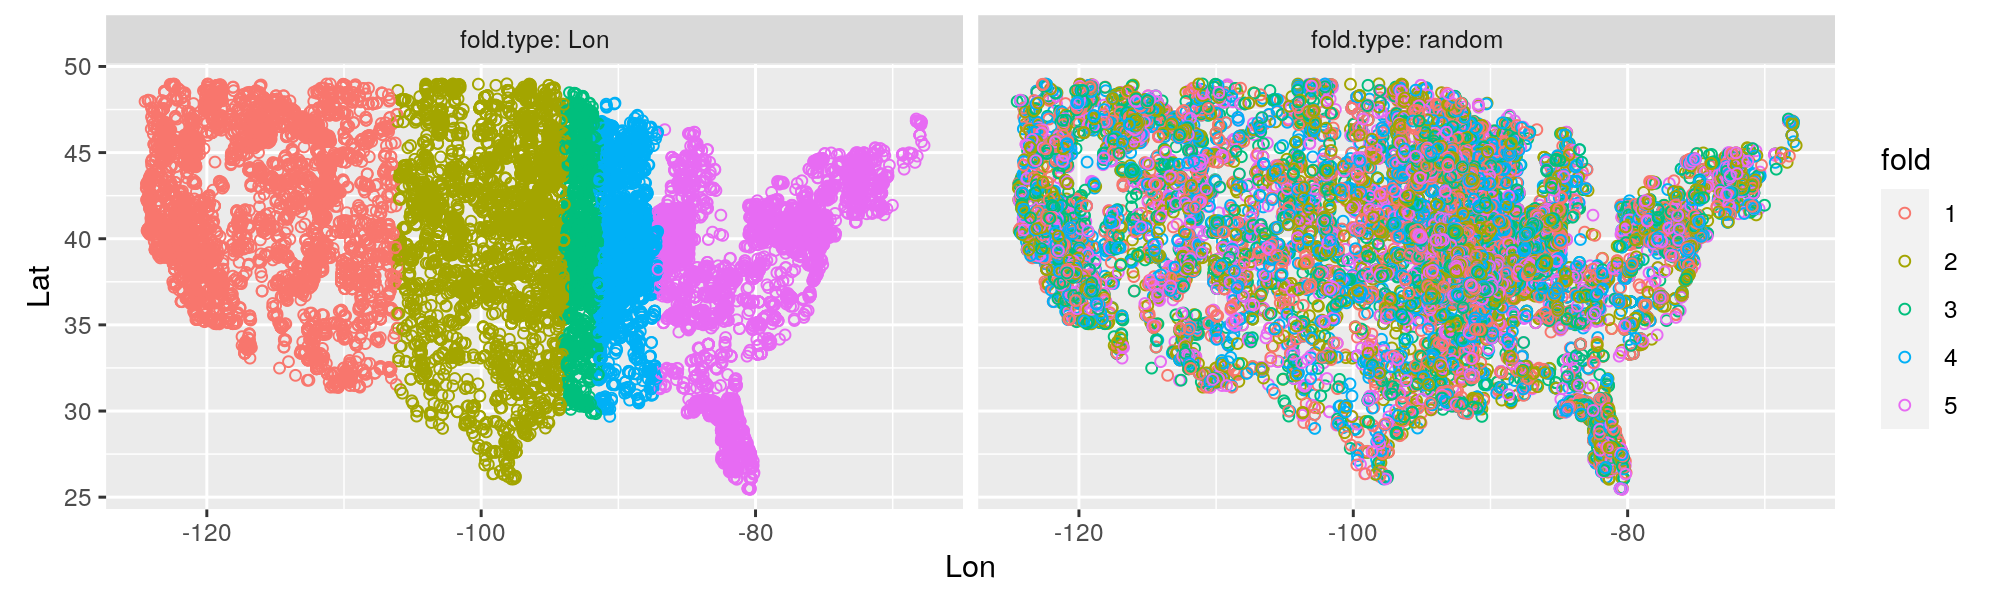
\includegraphics[width=0.9\textwidth]{figure-proda-cv-data-map}

  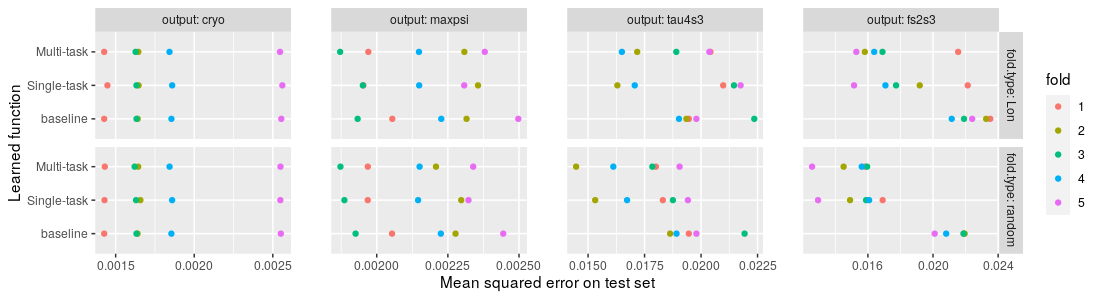
\includegraphics[width=0.9\textwidth]{figure-proda-cv-some-out}

  \begin{description}
  \item[Multi-task:] single neural network which predicts all 25 outputs.
  \item[Single-task:] 25 neural networks, each trained seperately to
    predict a single output.
  \item[baseline:] always predict the mean of the labels/outputs in
    the train set (feaureless, ignores inputs/features).
  \end{description}
  
\end{frame}

\section{Summary and quiz questions}

\begin{frame}
  \frametitle{Summary}
  Thanks for participating! We have studied
  \begin{itemize}
  \item Three examples of machine learning problems.
  \item Two kinds of problems, regression y=real number,
    classification y=integer category.
  \item Splitting a data set into train/test/subtrain/validation sets
    for learning hyper-parameters and evaluating prediction accuracy.
  \item Overfitting and how to avoid it by choosing hyper-parameters
    based on a validation set.
  \item Comparing prediction accuracy of learning algorithms with each
    other and to a featureless baseline.
  \end{itemize}
\end{frame}

\begin{frame}
  \frametitle{Quiz questions}
  \begin{itemize}
\item When using a design matrix to represent machine learning inputs,
  what does each row and column represent?
\item When splitting data into train/test sets, what is the purpose of
  each set? When splitting a train set into subtrain/validation sets,
  what is the purpose of each set?
\item In order to determine if any non-trivial predictive relationship
  between inputs and output has been learned, a comparison with a
  featureless baseline that ignores the inputs must be used. How do you compute
  the baseline predictions, for regression and classification
  problems?
\item How can you tell if machine learning model predictions are
  underfitting or overfitting?
\item Many learning algorithms require input of the number of
  iterations or epochs. For example in R the \texttt{nnet} function
  has the \texttt{maxit} argument and the \text{keras::fit} function
  has the \texttt{epochs} argument. How should this parameter be
  chosen?
  \end{itemize}
\end{frame}
 
\end{document}
